\documentclass[10pt]{article}

\usepackage{amsmath,amscd}
\usepackage{amssymb,array}
\usepackage{amsfonts,latexsym}
\usepackage{graphicx,subfig,wrapfig}
\usepackage{times}
\usepackage{psfrag,epsfig}
\usepackage{verbatim}
\usepackage{tabularx}
\usepackage[pagebackref=true,breaklinks=true,letterpaper=true,colorlinks,bookmarks=false]{hyperref}
\usepackage{ mathrsfs }

\DeclareMathOperator*{\rank}{rank}
\DeclareMathOperator*{\trace}{trace}
\DeclareMathOperator*{\range}{range}
\DeclareMathOperator*{\spn}{span}
\DeclareMathOperator*{\acos}{acos}
\DeclareMathOperator*{\argmax}{argmax}

\newcommand{\matlab}[1]{\texttt{#1}}
\newcommand{\setname}[1]{\textsl{#1}}
\newcommand{\Ce}{\mathbb{C}}

\newenvironment{mfunction}[1]{
\noindent
\tabularx{\linewidth}{>{\ttfamily}rX}
\hline
\multicolumn{2}{l}{\textbf{Function \matlab{#1}}}\\
\hline
}{\\\endtabularx}

\newcommand{\parameters}{\multicolumn{2}{l}{\textbf{Parameters}}\\}

\newcommand{\fdescription}[1]{\multicolumn{2}{p{0.96\linewidth}}{

\textbf{Description}

 #1}\\\hline}

\newcommand{\retvalues}{\multicolumn{2}{l}{\textbf{Returned values}}\\}
\def\0{\boldsymbol{0}}
\def\b{\boldsymbol{b}}
\def\bmu{\boldsymbol{\mu}}
\def\e{\boldsymbol{e}}
\def\u{\boldsymbol{u}}
\def\x{\boldsymbol{x}}
\def\v{\boldsymbol{v}}
\def\w{\boldsymbol{w}}
\def\N{\boldsymbol{N}}
\def\X{\boldsymbol{X}}
\def\Y{\boldsymbol{Y}}
\def\A{\boldsymbol{A}}
\def\B{\boldsymbol{B}}
\def\y{\boldsymbol{y}}
\def\cX{\mathcal{X}}
\def\transpose{\top} 

%\long\def\answer#1{{\bf ANSWER:} #1}
\long\def\answer#1{}
\newcommand{\myhat}{\widehat}
\long\def\comment#1{}
\newcommand{\eg}{{e.g.,~}}
\newcommand{\ea}{{et al.~}}
\newcommand{\ie}{{i.e.,~}}

\newcommand{\db}{{\boldsymbol{d}}}
\renewcommand{\Re}{{\mathbb{R}}}
\newcommand{\Pe}{{\mathbb{P}}}

\hyphenation{MATLAB}
\usepackage[margin=1in]{geometry}


\begin{document}

\title{
\vspace{-19mm}
Computer Vision (600.461/600.661)\\
Homework 6: Segmentation and Recognition}
\author{Greg Kiar}


\maketitle

\begin{enumerate}

\item \textbf{(25 points) Image Segmentation.}
\begin{enumerate}

%q1a
\item The code designed for this section is attached in the submitted folder and titled \texttt{spectral.m} and is accompanied by an example script that was used to run it, \texttt{hw6q1a.m}.

%q1b
\item The Spectral Clustering algoritm applied to the two applied images can be seen in the two figures below. As is clearly observed, the algorithm (applied to downsampled images) successfully segments foreground elements and background in both cases. Here, since no "\emph{ground truth}" exists, analysis of the success of these segmentations must be done qualitatively. For the case of the Night Sky image, the segementation very successfully differentiates features. We notice that the k-means algorithm is effective at grabbing smaller details of the image, but is also more senstive to noise in the image. For instance, the moon was not successfully recovered in all trials since the cluster centers are initially set randomly. In the case of the Penguin image, since the contrast between parts of the foreground and background is lower, parts of the foreground are segmented into the background region. In this case, both of the algorithms have difficulty detecting the head of the penguin. That being said, the method still successfully identifies the large forground object effectively.
\begin{figure}[h!] 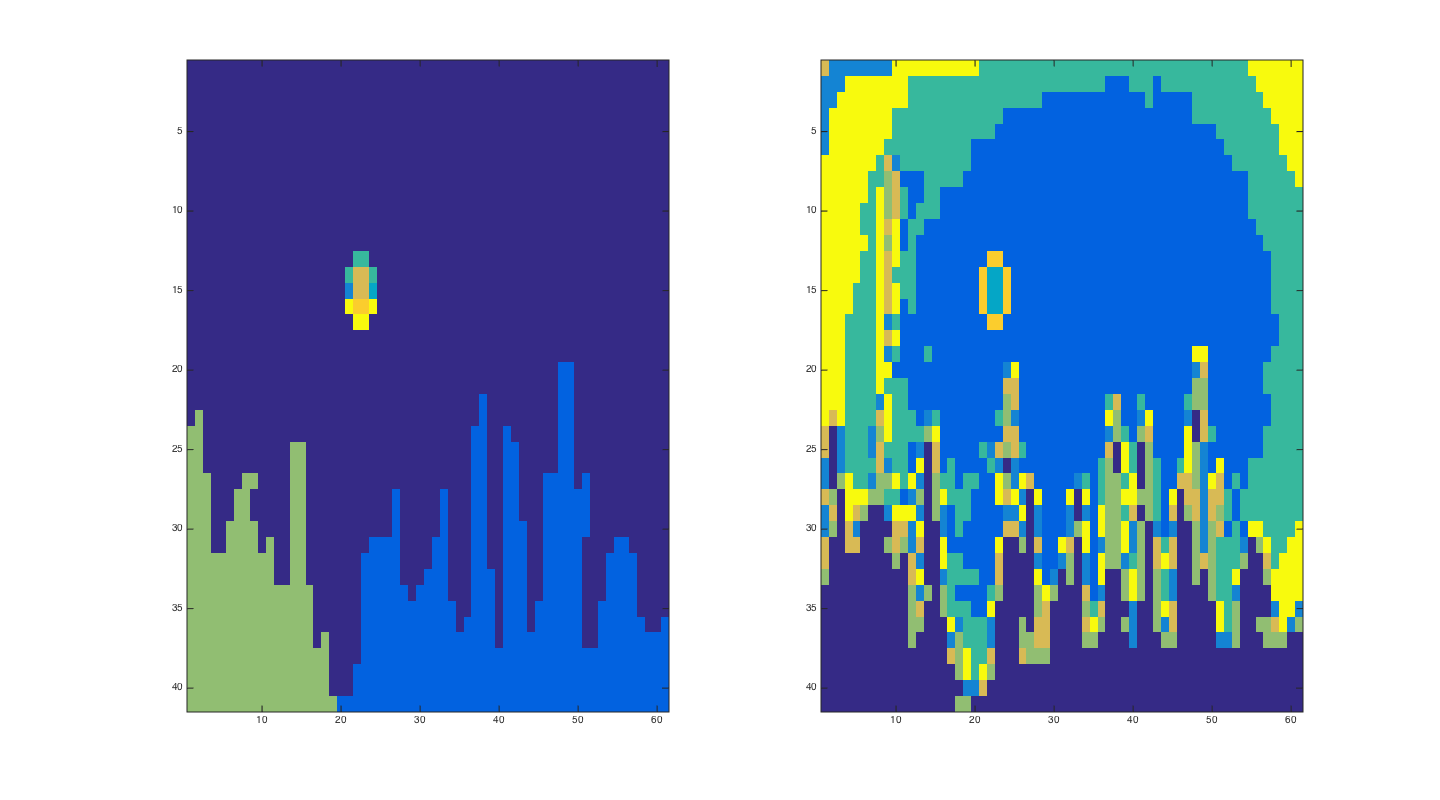
\includegraphics[scale=0.35]{hw6q1b1.png} \caption[h1]{Night Sky image segmentation using Spectral Clustering (left) and K-means (right)} \end{figure}
\begin{figure}[h!] 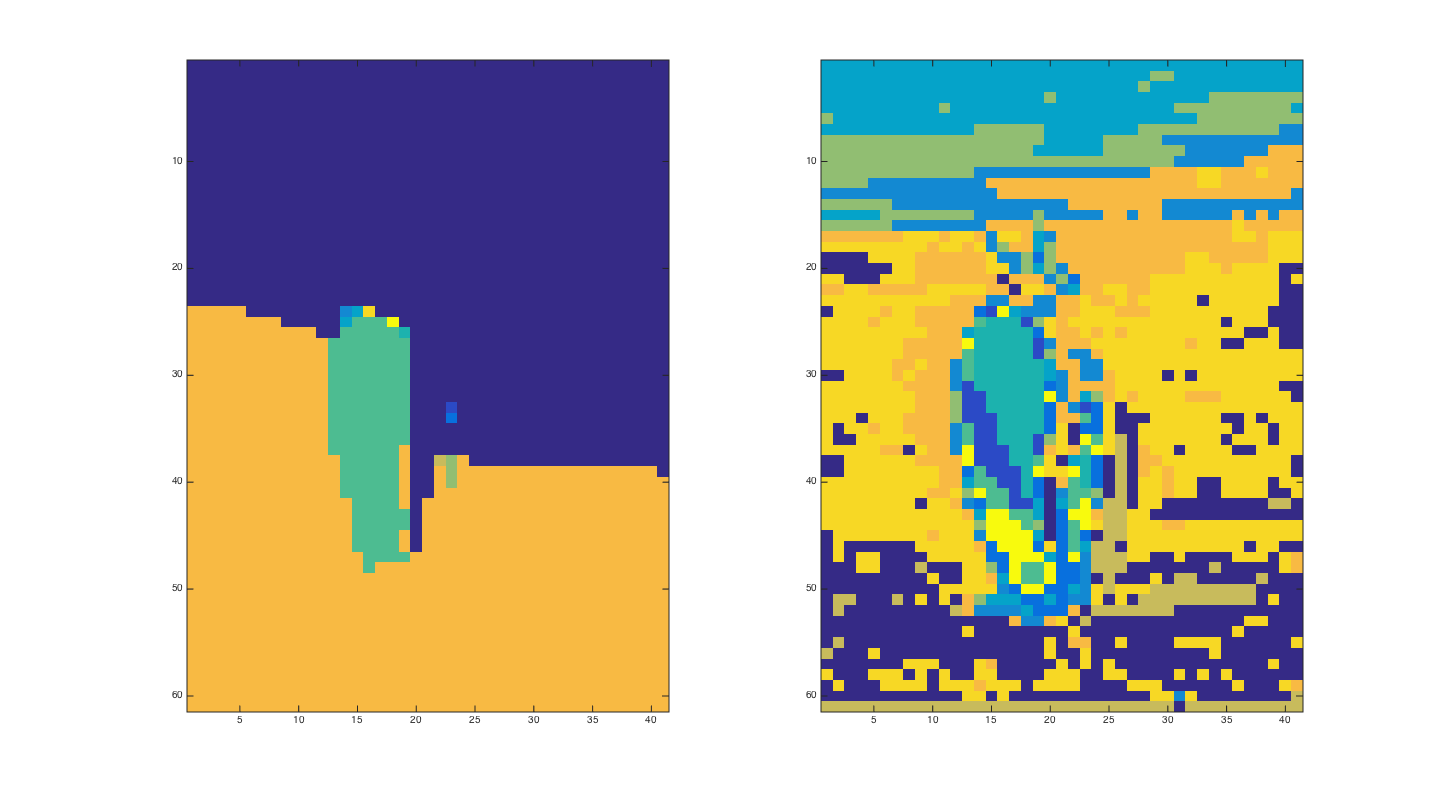
\includegraphics[scale=0.35]{hw6q1b2.png} \caption[h2]{Penguin image segmentation using Spectral Clustering} \end{figure} \\ \newpage

%q1c
\item Applying Colour-based segmentation using the k-means and spectral clustering algorithms developed earlier, we can also note successful identification of regions using these methods. In the first, chick, image, a figure below shows both the spectral clustering and k-means methods for segmentation on both the $(h,s)$ and $(r,g)$ images. We can see that for this image, with both colour schemes, the spectral clustering algorithm out-performs k-means. Between colour schemes, we notice very little difference in result here. A possible reason for the better performance of spectral clustering is that the cluster centers were picked based on optical connectivity, as opposed to randomly allocated. With so many regions, k-means would be hard pressed with random initial seed locations to successfully identify all of the regions.
\begin{figure}[h!] 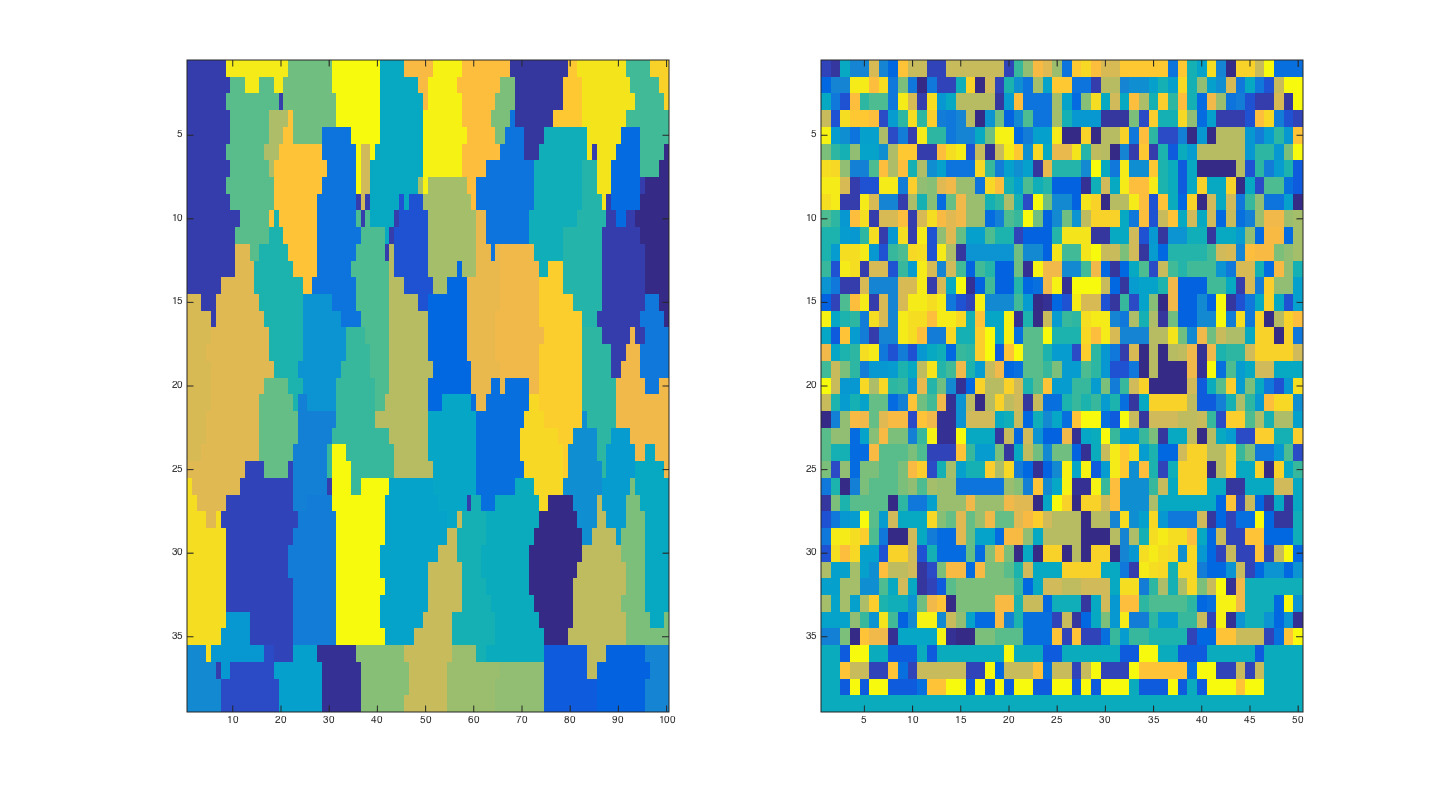
\includegraphics[scale=0.35]{hw6q1c1.png} 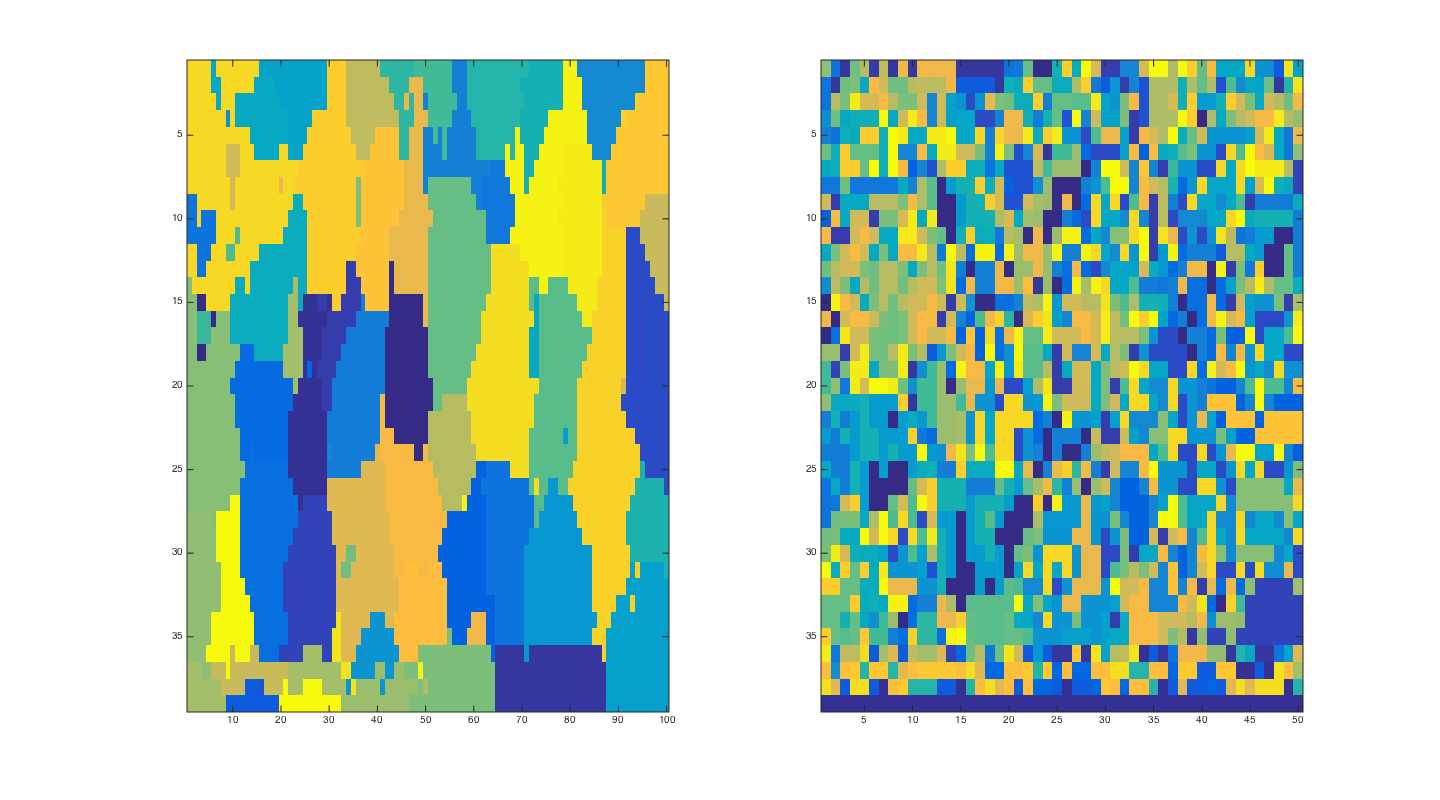
\includegraphics[scale=0.35]{hw6q1c2.png} \caption[h3]{Chick Image segmentation using Spectral Clustering (left) and K-means (right) for $(r,g)$ (top) and $(h,s)$ (bottom) color formats} \end{figure} \\

Looking at the image of the building, we see the opposite result as was displayed above. For this case, the k-means algorithm performs much better than the spectral clustering. In this case, the result could be due to the fact that there are many edges and boundaries, so the connectivity based clustering algorithm cannot successfully identify regions to connect to one another. A possible solution to this, in future iterations, could be to increase the connectivity used by spectral clustering from 8-connectivity to be a wider region. As in the case above, the image colour scheme didn't have a significant effect on the result.
\begin{figure}[h!] 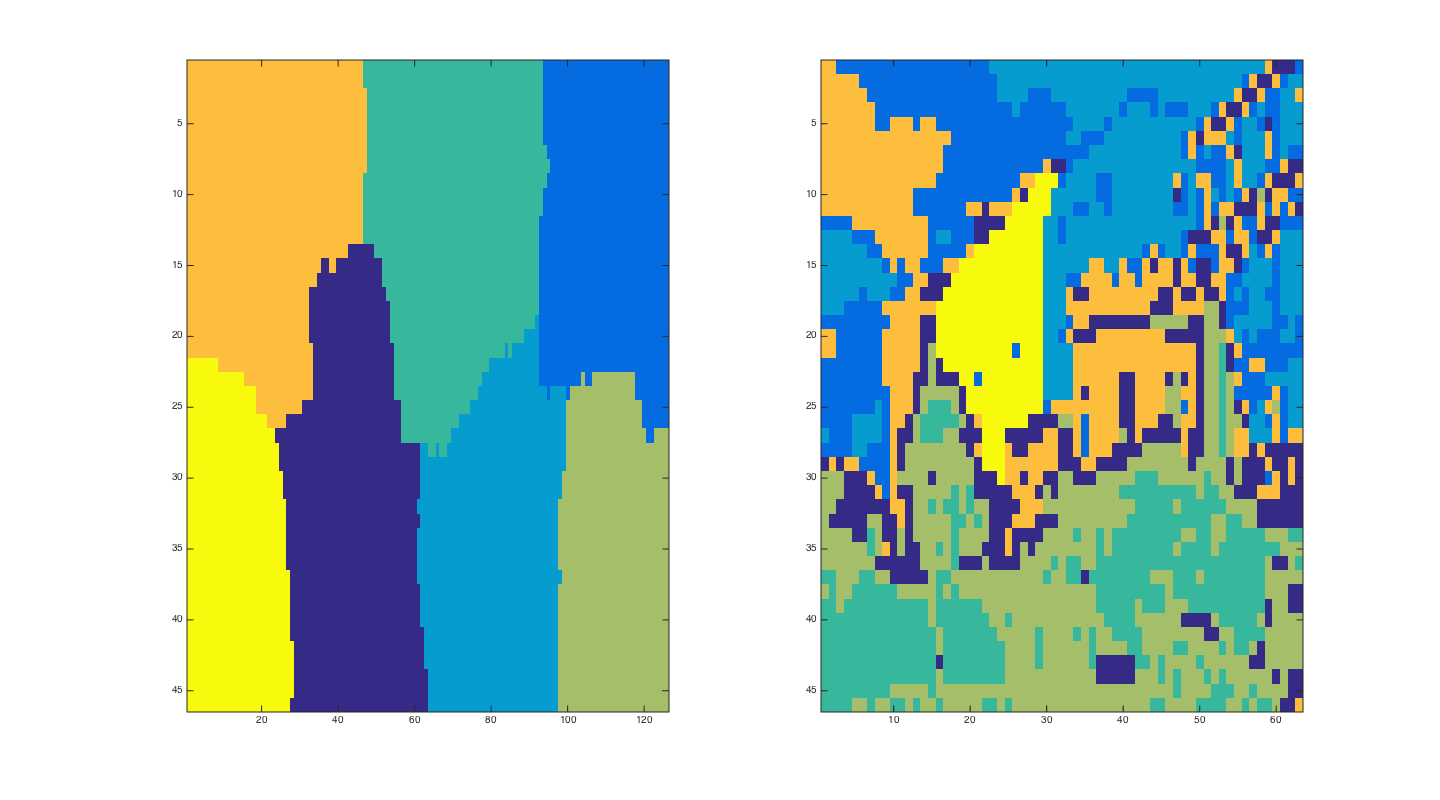
\includegraphics[scale=0.35]{hw6q1c3.png} 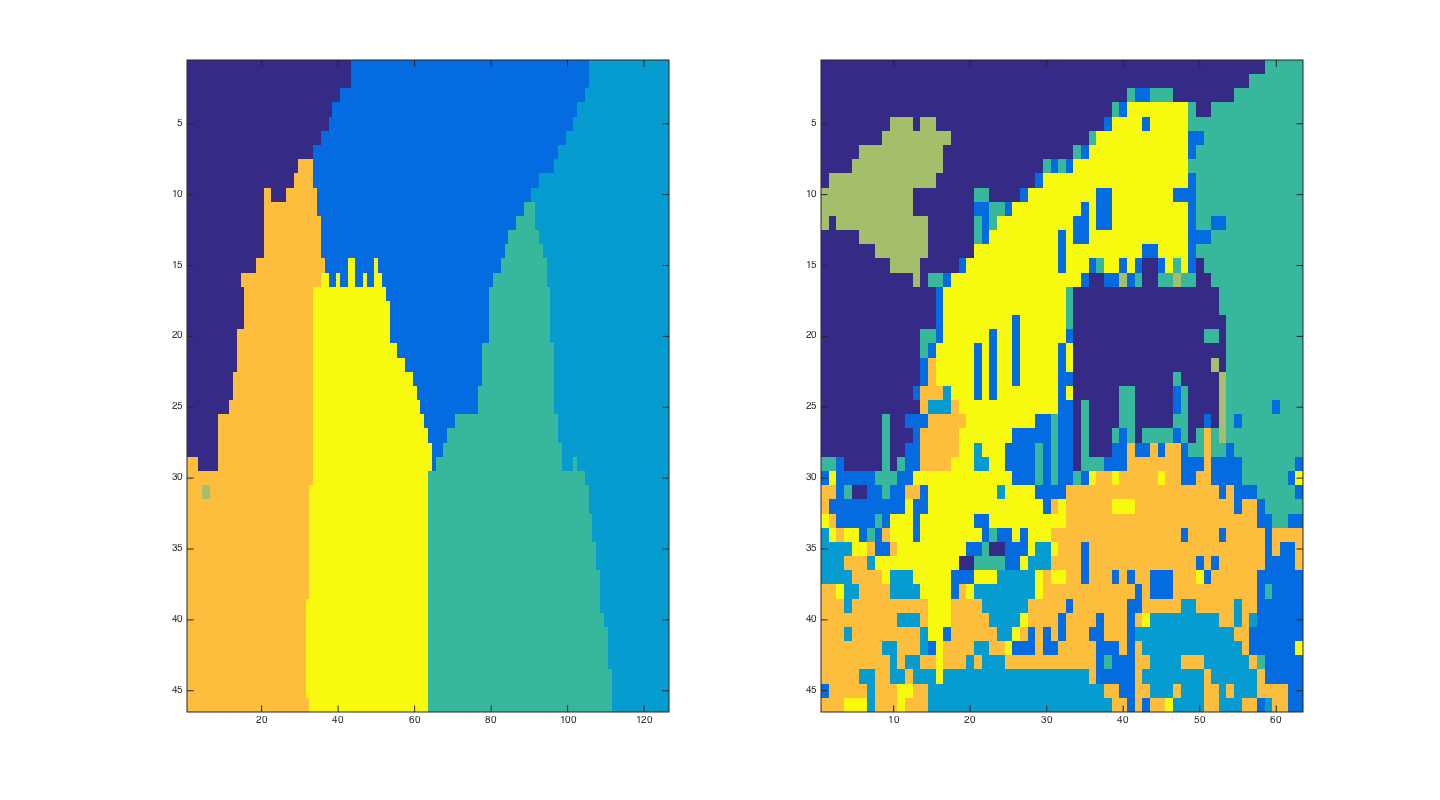
\includegraphics[scale=0.35]{hw6q1c4.png} \caption[h4]{Building Image segmentation using Spectral Clustering (left) and K-means (right) for $(r,g)$ (top) and $(h,s)$ (bottom) color formats} \end{figure} \\ \\
\newpage
\end{enumerate}
\clearpage
\item \textbf{(25 points) Object Recognition.}
\begin{enumerate}

%q2a
\item This task was removed from the homework.
\item The code designed for this section is attached in the submitted folder and titled \texttt{hw6q2b.m}. A large portion of this code was copied from the \texttt{exercise1.m} script that accompanied the software package used.
\end{enumerate}

\end{enumerate}
\end{document}
